%-------------------------------------------------------------
% Language
% Use the option "language=EN" to set the beamer theme in English. Use
% the option "language=ES" to set the beamer theme in Spanish.

% Colors
% Use the option "color=white" to set the background in white and the
% bottom bar in blue. Use the option "color=blue" to set the
% background in blue and the bottom bar in white. Use the option
% "color=blue2" to set the background in blue and the bottom bar in
% blue.

% Font Color
% Use the option "fontc=black" to set the font color in black. If this
% argument is not given the default color is set depending of the
% color scheme selected.

% Credits: https://github.com/alejogm0520 & Samuel Plazas Escudero
%-------------------------------------------------------------

%--Principal packages
\documentclass[aspectratio=43,8pt]{beamer} % 4:3, can be 16:9
\usetheme[language=ES, color=white]{EAFIT}
\usepackage[spanish]{babel}
\decimalpoint % All decimal numbers with point
\usepackage[utf8]{inputenc}
\selectlanguage{spanish}
\usepackage{amsmath,amsfonts,amssymb,cancel,physics} % Equations
\usepackage{verbatim} % Environments, \begin{comment}
%--Arial
\usepackage{helvet}
\renewcommand{\familydefault}{\sfdefault}
%--Beamer packages
\usepackage{tikz} % For making vectorized figures, arrows
\usepackage{ifthen} % For specifying conditionals for sections
\usepackage{ragged2e}\justifying % Whole text justified, except enumerate: add \justifying
\usepackage{xcolor}
\usepackage{multicol} % Multiple columns in one frame
%--Tables-Figures
\renewcommand\spanishtablename{Tabla}
\usepackage{booktabs,multirow} % Bookstyle tables
%-Figure label
\usepackage[labelsep=period,justification=justified,format=plain]{caption} % Dot instead of colon and justified caption
%--Figure
\usepackage{graphicx,subcaption} % Figures and subfigures
\graphicspath{{media/}} % Media rute
%-Figure-Table on top
\usepackage{float} % Allows to put H instead of ht
\setbeamertemplate{caption}[numbered] % Numbered captions
%---------TOC
\setbeamertemplate{section in toc}[sections numbered]
\setbeamertemplate{subsection in toc}[subsections numbered]
\setbeamerfont{section in toc}{size=\small}
\setbeamerfont{subsection in toc}{size=\footnotesize}
\setbeamertemplate{subsection in toc}{\leavevmode\leftskip=3.2em\rlap{\hskip-2em\inserttocsectionnumber.\inserttocsubsectionnumber}\inserttocsubsection\par} % Indented subsection
\setcounter{secnumdepth}{1}
%---------Cite
\usepackage{bibentry} % Full cite foot
\nobibliography* % Full cite foot
% Or: \setbeamertemplate{bibliography item}[text]
\setbeamertemplate{bibliography item}{\insertbiblabel}
%---------Footnotes
\setbeamercolor{footnote}{fg=white}
\setbeamercolor{footnote mark}{fg=.} % Takes the color depending on the circumpstance
\setbeamercolor{bibliography entry author}{fg=white} % Allows to have white footnote bibs
\setbeamertemplate{footnote}
{
  \hspace*{-1cm} % Horizontal movement
  \vspace*{-2.88cm} % Vertical movement
  \parbox[c][3.4cm]{10.6cm}{\tiny\noindent\insertfootnotemark\insertfootnotetext} % b: bottom, height: 3.3cm, horizontal length: 10.6cm (max horizontal)
% If there are problems, put -2.87cm and 3.3cm
}
\renewcommand{\footnoterule}{\kern -3pt \hrule width \textwidth height 0pt\kern 3pt} % No footnoterule
%------------------------------------
%---------Numbered Slides and Sections
\setbox0=\hbox{\subsecname\unskip}\ifdim\wd0=0pt\else%
 ~--~\insertsubsectionhead
\fi
%------Numbering section: title in bold, centered and with a line
\newcommand{\numb} 
{
  \setbeamertemplate{frametitle}
  {
    \ifx\insertsubsection\empty % No subsection
         \bfseries\thesection.~\insertframetitle~\color{black}\par\vskip-5pt\hrulefill % \centering
    \else % subsection
         \bfseries\thesection.~\insertframetitle~\color{black}\par\vskip-9pt\hrulefill\par\vskip3pt{\large\thesection.\thesubsection~\insertframesubtitle} % Subsection with smaller size;
    \fi
  }
}
%------No numbering section: title in bold, centered and with a line
\newcommand{\nonumb}
{
  \setbeamertemplate{frametitle}{\bfseries\color{black}\centering\insertframetitle\par\vskip-6pt\hrulefill}
}
%------------------------------------
%--No hyphenation on text
\tolerance=1
\emergencystretch=\maxdimen
\hyphenpenalty=10000
\hbadness=10000
%------------------------
%---------Itemize justified in beamer
\makeatletter
\renewcommand{\itemize}[1][]{
  \beamer@ifempty{#1}{}{\def\beamer@defaultospec{#1}}
  \ifnum \@itemdepth >2\relax\@toodeep\else
    \advance\@itemdepth\@ne
    \beamer@computepref\@itemdepth % Sets \beameritemnestingprefix
    \usebeamerfont{itemize/enumerate \beameritemnestingprefix body}
    \usebeamercolor[fg]{itemize/enumerate \beameritemnestingprefix body}
    \usebeamertemplate{itemize/enumerate \beameritemnestingprefix body begin}
    \list
      {\usebeamertemplate{itemize \beameritemnestingprefix item}}
      {\def\makelabel##1{
          {
            \hss\llap{{
                \usebeamerfont*{itemize \beameritemnestingprefix item}
                \usebeamercolor[fg]{itemize \beameritemnestingprefix item}##1}}
          }
        }
      }
  \fi
  \beamer@cramped
  \justifying % Justified itemize
  \beamer@firstlineitemizeunskip
}
\makeatother
%------------------------
%---------Get current section name for showing it at its begining
\usepackage{nameref}
\makeatletter
\newcommand*{\currentname}{\@currentlabelname}
\makeatother
%---------Shows in which section we are at the begining of each one
\AtBeginSection[]
{
\begin{frame}[plain,noframenumbering]
  \begin{beamercolorbox}[ht=\paperheight,wd=\paperwidth, center]{Portada}
    \begin{center}\textbf{\LARGE \currentname}\end{center} % Leave the next space mandatorily

    \vspace{0.44\paperheight}
  \end{beamercolorbox}
\end{frame}
}
%-------------------(constantly being edited)------------------

%---------TEXTBLOCKS-GRID 
\usepackage[absolute,overlay,showboxes]{textpos}
%\usepackage[texcoord,grid,gridunit=mm,gridcolor=red!10,subgridcolor=green!10]{eso-pic} % Helping grids, comment when publishing
%---------COLOR DEFINITIONS
\definecolor{azure(colorwheel)}{rgb}{0.0, 0.5, 1.0} % Define colors here


%%%%%%%%%%%%%%%%%%%%%%%
%Start of the Document%
%%%%%%%%%%%%%%%%%%%%%%%

%---------COVER PAGE

\title{LA FÍSICA DEL GOLF{}}
\author{\normalfont\large\texorpdfstring{Presentado por:\\ Juan S. Cárdenas Rodríguez\\ Mariana Escobar Quiceno \\ David Plazas Escudero\\[2ex] Profesora: \\Luz Marleny Morales Mira}{}} % PA

\def\departamento{Departamento de Ciencias Físicas}
\def\escuela{Escuela de Ciencias}
\def\materia{Física I}
\def\eafit{Universidad EAFIT}
\def\fecha{2017}
% to add more def, search for "Dirección" in beamerthemeEAFIT.sty



%\includeonly{c/ex}
\begin{document}

\nonumb % Not numbered titles
\begin{frame}
% Portada Inspira Crea Transforma
\end{frame}
%%%%%%%%%%%%%%%%%%%%%%%%%%%%%%%%%%%%%%%%%%%%%%%%%%%%%%%%%%%%%%%%%%%%%%%%%%%%
\begin{frame}
\begin{center}
  \titlepage % Cover page
\end{center}
\end{frame}
%%%%%%%%%%%%%%%%%%%%%%%%%%%%%%%%%%%%%%%%%%%%%%%%%%%%%%%%%%%%%%%%%%%%%%%%%%%%
\begin{frame}{CONTENIDO}
\begin{multicols}{2}
  \tableofcontents
\end{multicols}
\end{frame}
\numb % Numbered titles
%\include{ex_beamer_teams} % Comment when publishing
\section{OBJETIVOS}
  \label{obj}
  \subsection{GENERAL}
    \begin{frame}{OBJETIVOS}
      \framesubtitle{GENERAL}
      Analizar la cinemática, dinámica traslacional y rotacional en el golf.
      \begin{figure}[H]
        \centering
        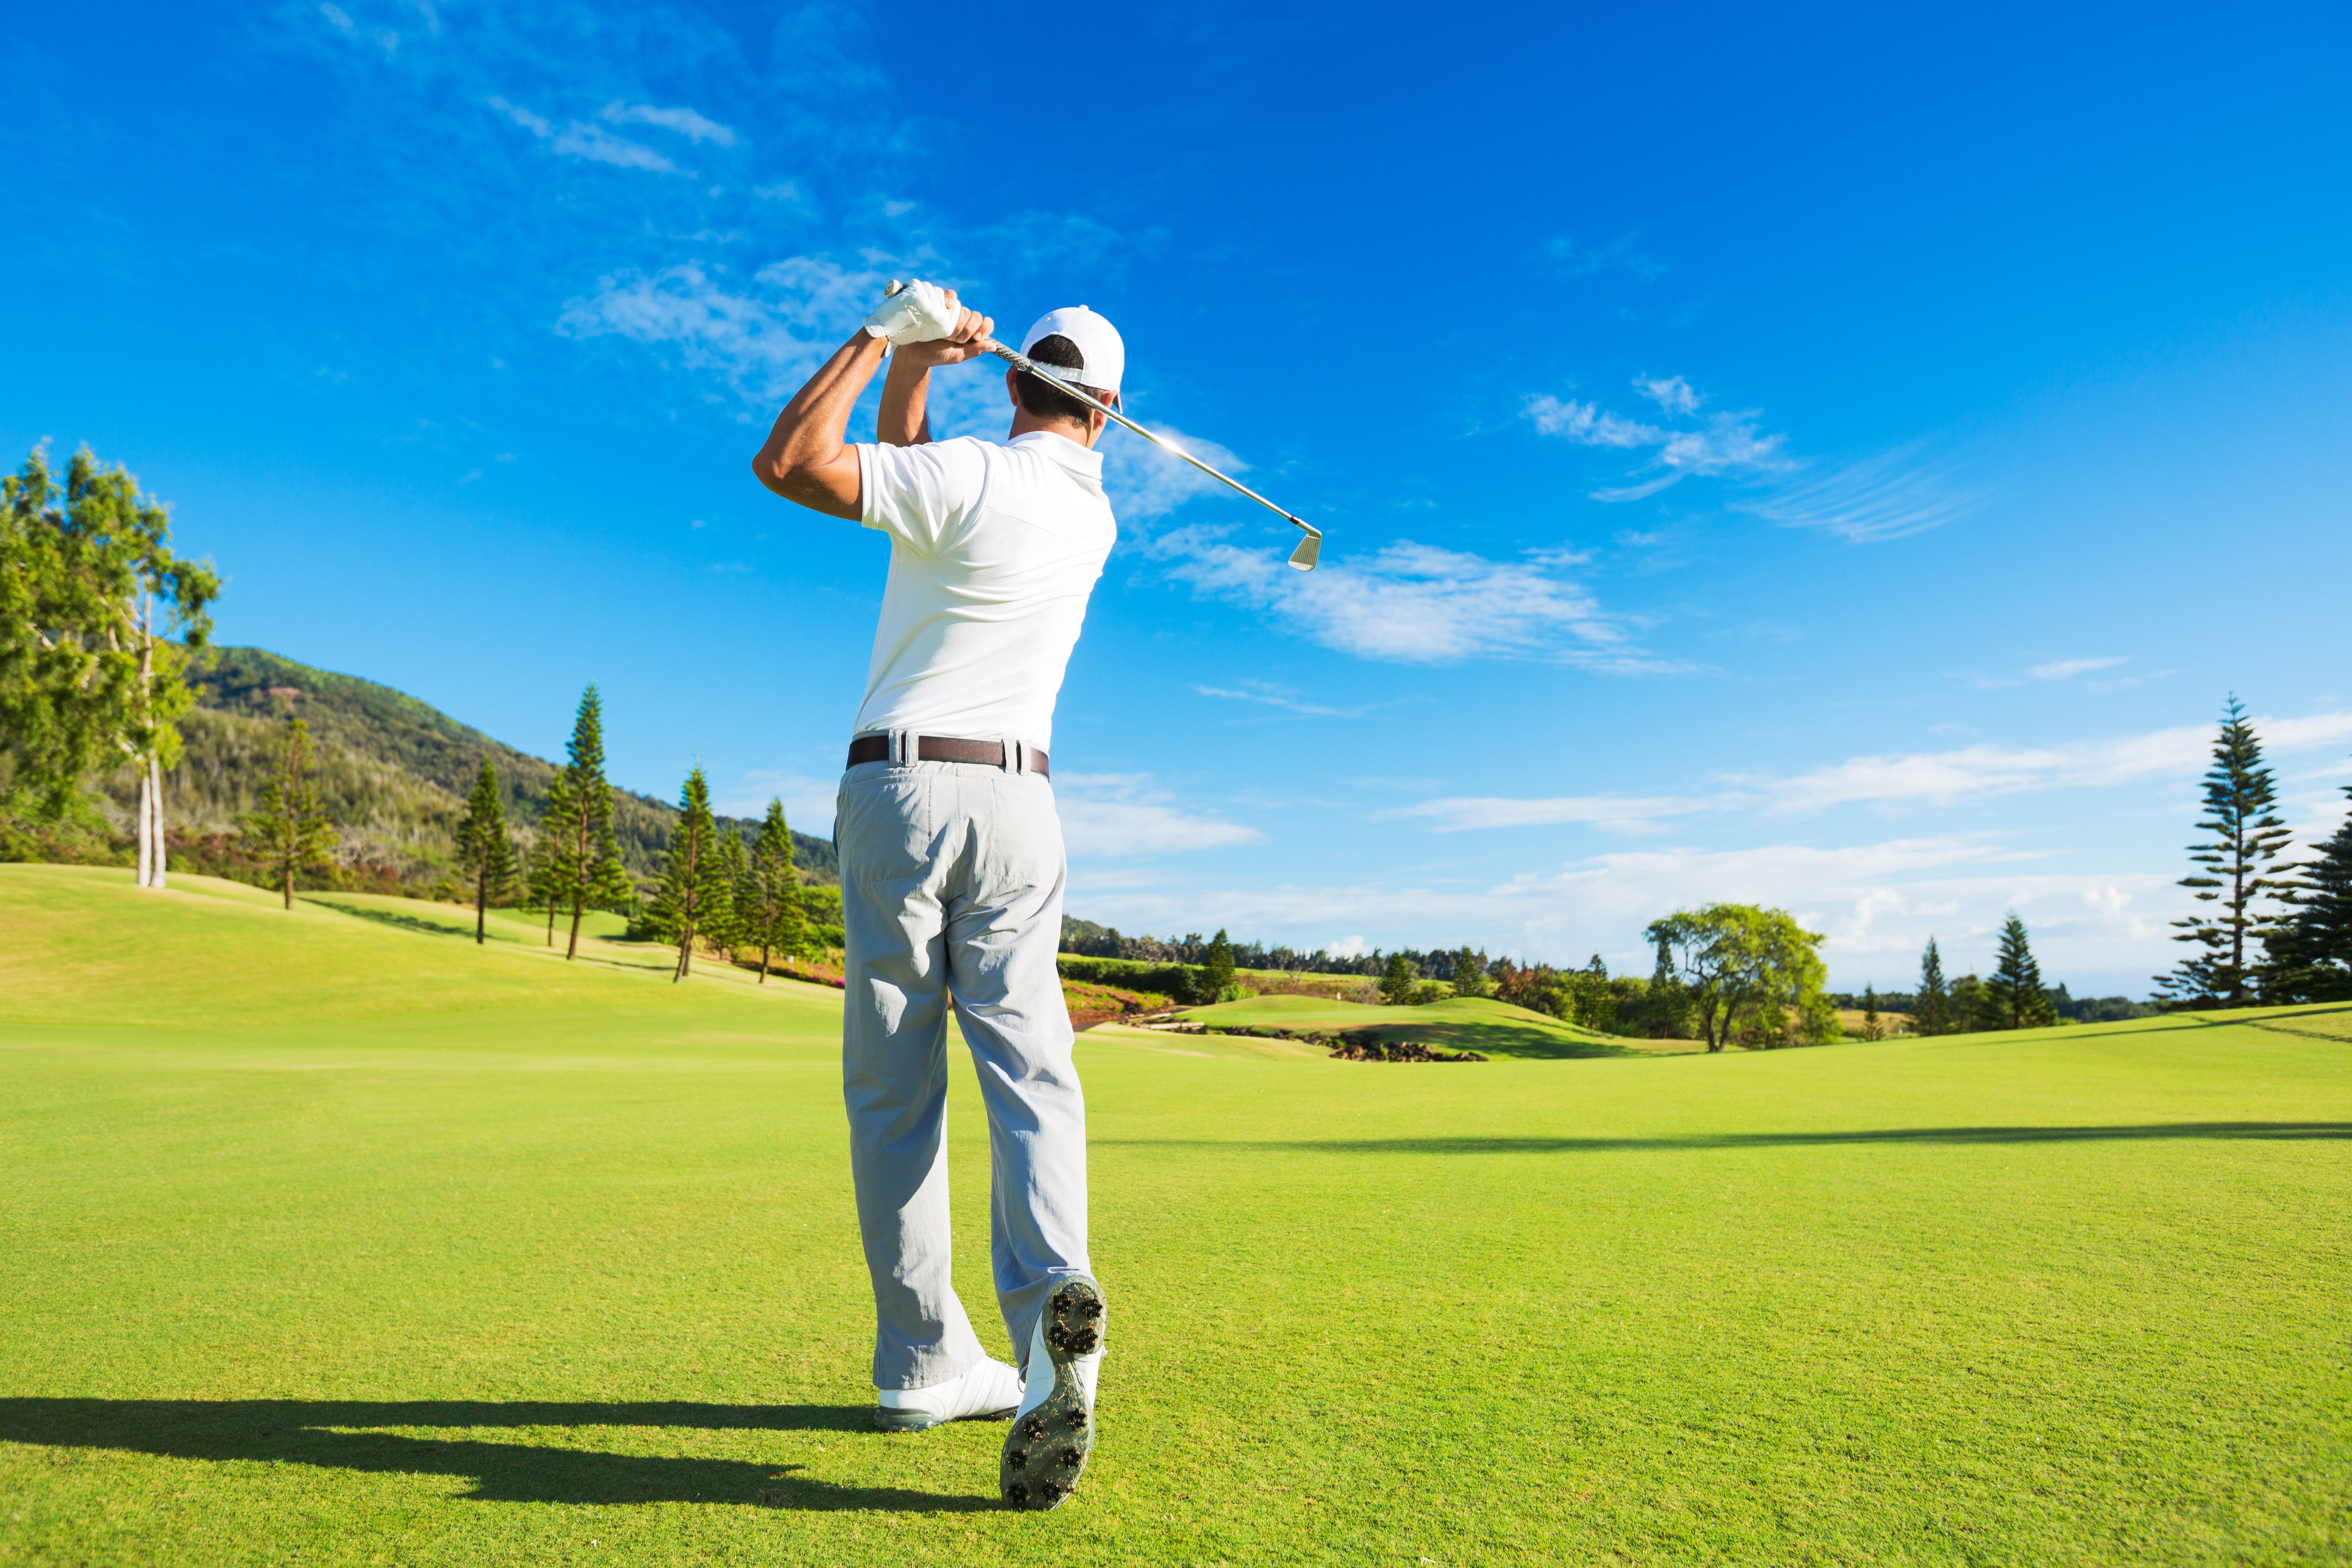
\includegraphics[scale = 0.03]{NiceSwing.jpg}
        \caption{Jugador de golf\footnotemark{}.}
      \end{figure}
      \footnotetext{\bibentry{NiceSwing}.}
    \end{frame}

  \subsection{ESPECÍFICOS}
  \begin{frame}{OBJETIVOS}
    \framesubtitle{ESPECÍFICOS}
    \begin{itemize}
      \item Describir las características recomendadas para los jugadores de golf.
      \item Explicar las funciones e implicaciones físicas de los accesorios presentes en un juego de golf.
      \item Explicar la forma en que los fenómenos físicos afectar la técnica de los jugadores de golf.
      \item Explicar el impacto físico de los implementos utilizados en el golf.
    \end{itemize}
    


  \end{frame}
\section{CONTEXTUALIZACIÓN}
\subsection{Historia}
\begin{frame}{CONTEXTUALIZACIÓN}
\framesubtitle{Historia y objetivo}
	El objetivo del juego es introducir una bola en hoyos que están distribuidos en el campo con el menor número de golpes. El juego que hoy conocemos fue inventado por los escoceses entre el siglo XIV y el XV \footnote{\bibentry{history}}.
    \begin{figure}[H]
      \centering
      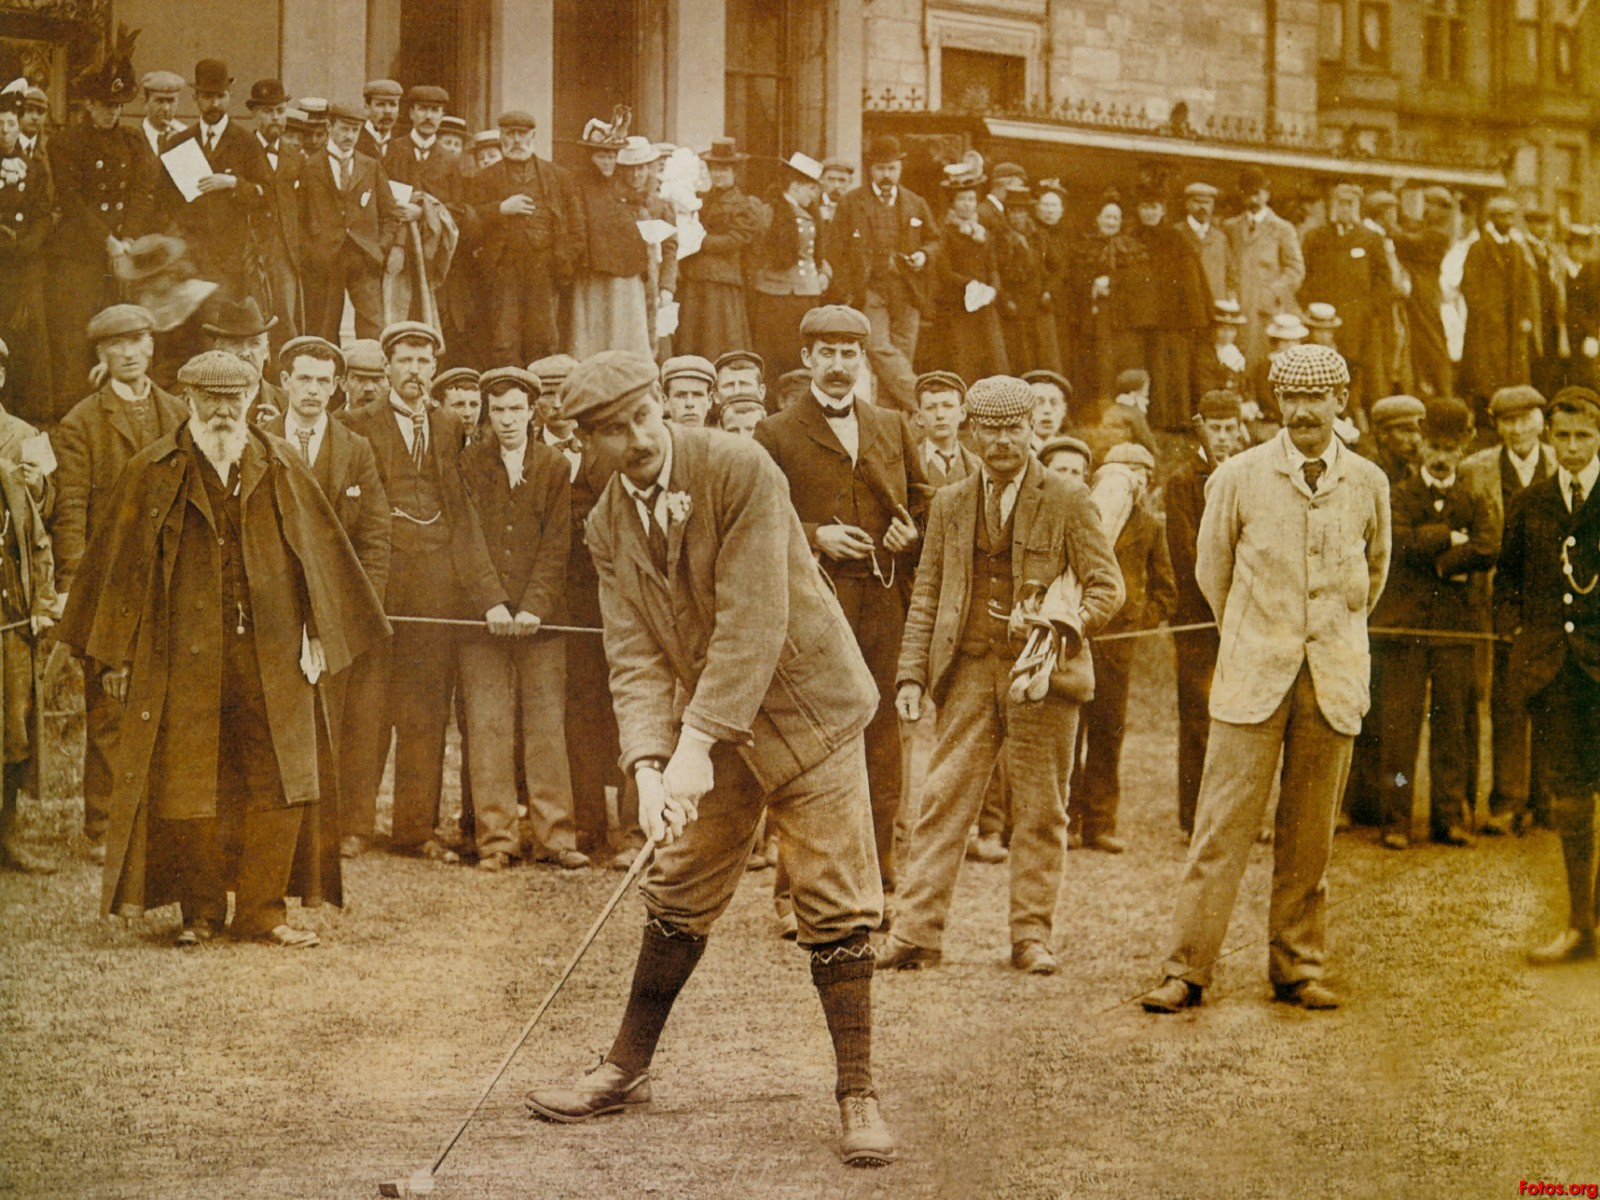
\includegraphics[scale = 0.1]{historia.jpg}
      \caption{Juego de golf, siglo XX\footnotemark{}.}
	\end{figure}
\footnotetext{\bibentry{imgHist}}
\end{frame}
%%%%%%%%%%%%%%%%%%%%%%%%%%%%%%%%%%%%%%%%%
\subsection{Sobre el Campo de Golf}
\begin{frame}{CONTEXTUALIZACIÓN}
\framesubtitle{Sobre el Campo de Golf}
	\begin{figure}[H]
      \centering
      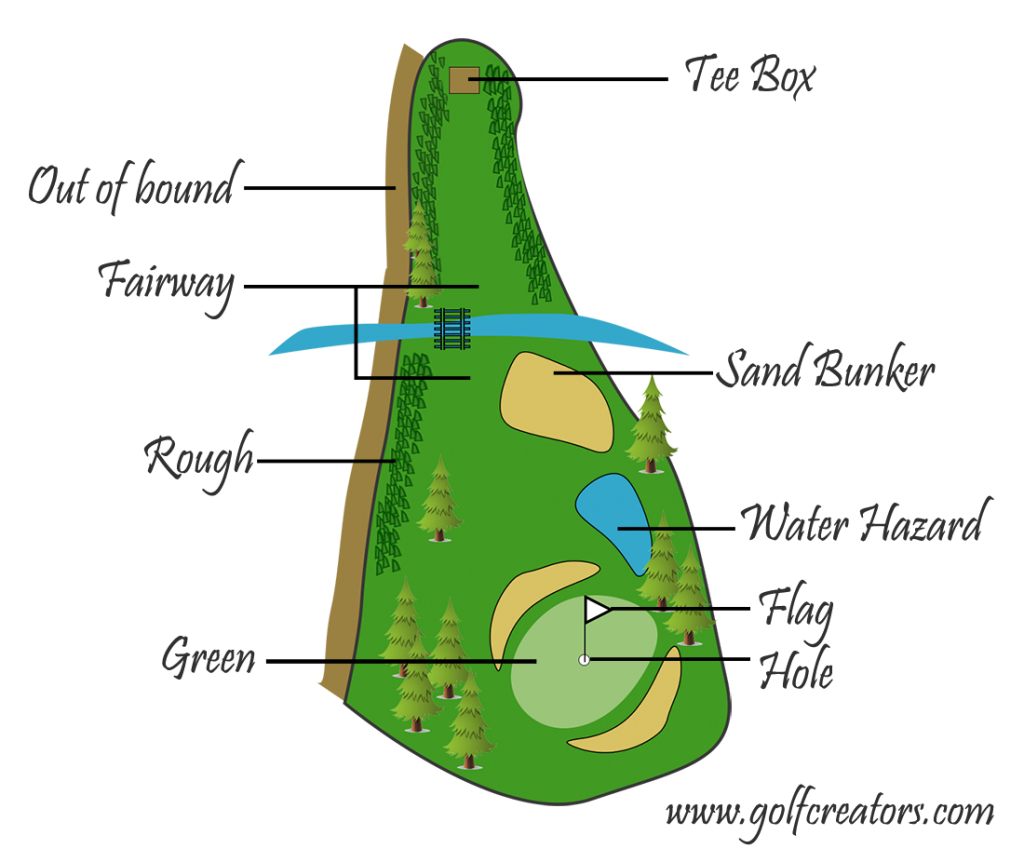
\includegraphics[scale = 0.2]{GolfCourse.png}
      \caption{Campo de Golf.}
	\end{figure}
\end{frame}
%%%%%%%%%%%%%%%%%%%%%%%%%%%%%%%%%%%%%%%
\subsection{Introducción}
\begin{frame}{CONTEXTUALIZACIÓN}
\framesubtitle{Introducción}
¿Cómo cambia el movimiento de un objeto cuando está en un fluido?\\
\url{https://www.khanacademy.org/computing/computer-programming/programming-natural-simulations/programming-forces/a/air-and-fluid-resistance}
\end{frame}



\section{GLOSARIO}
\begin{frame}{GLOSARIO}
	\begin{itemize}
		\item Tee (de salida): Lugar del hoyo de golf donde los golfistas comienzan el juego en cada hoyo.
  	    \item Down swing: Bajada del palo que comienza desde lo alto del back swing hasta el momento del impacto de la cara del palo en la bola de golf.
        \item Backswing: Es la parte del swing de golf en la que elevamos el palo. Comienza cuando arrancamos la cabeza del palo en el inicio del swing y termina en lo alto de la subida del palo.
        \item Swing: Movimiento que empleamos para golpear la bola de golf 
        
            \item Grip (mango): Mango de goma situado en la varilla de los palos de golf, con la finalidad de facilitar su agarre. Existen diferentes tipos y grosores, en función de los jugadores o jugadoras a los que van destinados\footnote{\bibentry{bworld}}.
        \item Número de Reynolds: Se utiliza para estudiar la manera en que se comporta el fluido al rededor de un objeto en movimiento; en particular, para determinar si el flujo es laminar o turbulento\footnote{\bibentry{reynolds}}.
	\end{itemize}
\end{frame}
%%%%%%%%%%%%%%%%%%%%%%%%%%%%%%
\begin{frame}{GLOSARIO}
\begin{itemize}
			\item Hook: Efecto pronunciado hacia la izquierda que toma la bola de golf durante el vuelo, a consecuencia de llegar la cara del palo cerrada en el momento del impacto.
            \item Slice: Efecto pronunciado hacia la derecha que toma la bola de golf durante el vuelo, a consecuencia de llegar la cara del palo abierta en el momento del impacto.
            \item Backspin: Efecto de retroceso que se imprime al golpear la bola. Cuando impacta en el green, regresa en sentido opuesto a la trayectoria del golpe.
            \item Overspin: opuesto al backspin\footnote{\vspace{-0.3cm}\bibentry{bworld}}.
\end{itemize}
    \begin{figure}[H]
      \centering
      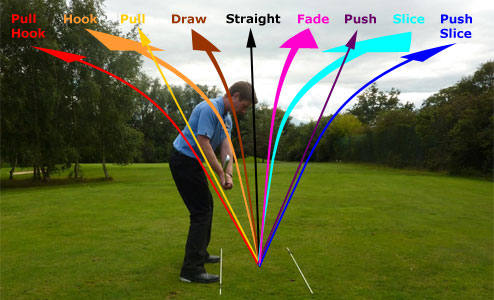
\includegraphics[scale = 0.35]{Spin_Shots.jpg}
      \caption{Tipos de tiro en el golf.}
	\end{figure}
\end{frame}










\section{DINÁMICA TRASLACIONAL}
\subsection{Arrastre y levantamiento}
\begin{frame}{DINÁMICA TRASLACIONAL}
\framesubtitle{Arrastre y levantamiento}
	La resistencia del aire se puede descomponer en las componentes x y y del movimiento y
nombrarlas como una fuerza de arrastre y una de levantamiento respectivamente.
	\begin{figure}[H]
      \centering
      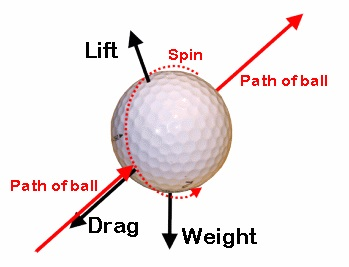
\includegraphics[scale = 0.5]{forces.jpg}
      \caption{Diagrama de cuerpo libre para una bola de golf\footnotemark{}.}
    \end{figure}
     \footnotetext{\bibentry{forces}.}
\end{frame}

%%%%%%%%%%%%%%%%%%%%%%%%%%%%%%%%%%%%%%%%%%%%%%%%%%%%%%%%%%%%%%%%%%%%%%%%

\subsection{Números de Reynolds}
\begin{frame}{DINÁMICA TRASLACIONAL}
\framesubtitle{Números de Reynolds}
	Depende del diametro del objeto de estudio ($D$), la viscocidad del fluido ($\mu$), la densidad del fluido ($\rho$) y la velocidad del fluido ($v$).
	\begin{equation}
		Re=\frac{\rho vD}{\mu}
	\end{equation}
    \begin{figure}[H]
      \centering
      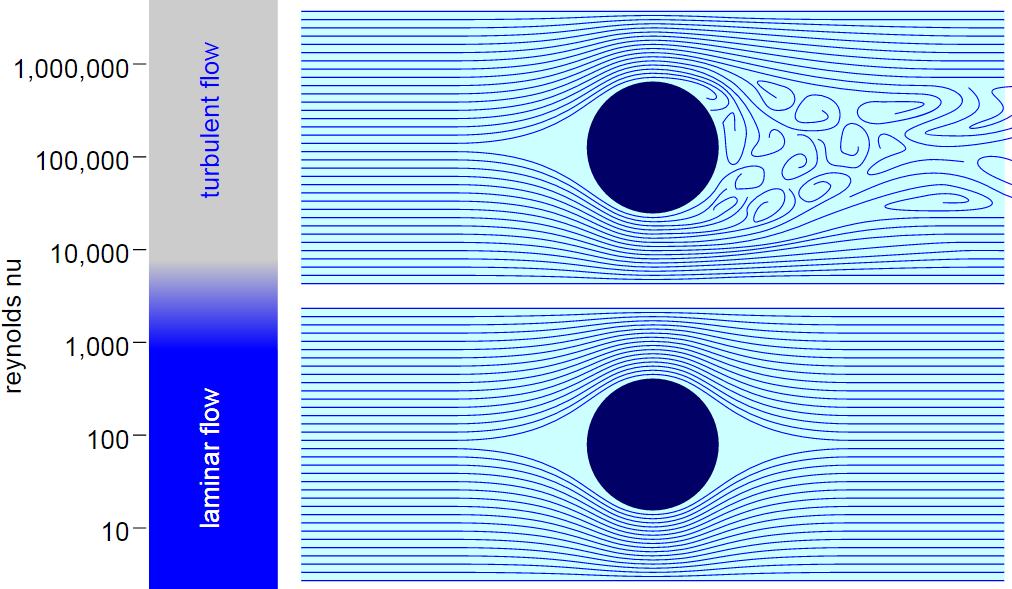
\includegraphics[scale = 0.25]{Flow-Regime.png}
      \caption{Comportamiento del fluido de acuerdo a los valores del número de Reynolds.\footnotemark{}.}
    \end{figure}
     \vspace{-1cm}\footnotetext{\bibentry{reynolds2}.}
   	\end{frame}
    
%%%%%%%%%%%%%%%%%%%%%%%%%%%%%%%%%%%%%%%%%%%%%%%%%%%%%%%%%%%%%%%%%%%%%

\subsection{Crisis de arrastre}
\begin{frame}{Dinámica traslacional}
\framesubtitle{Crisis de arrastre}
	Al analizar la gráfica de fuerza de arrastre contra número de Reynolds se obtiene un resultado algo contradictorio para la época.
	\begin{figure}[H]
      \centering
      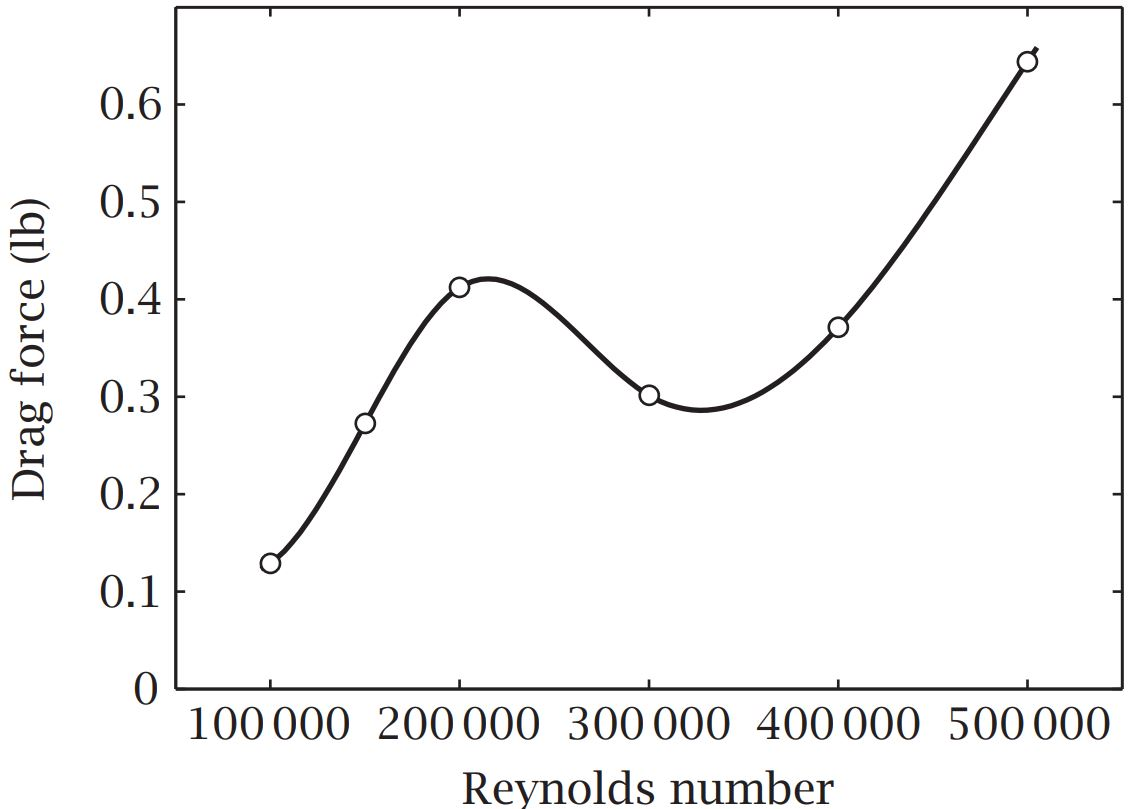
\includegraphics[scale = 0.2]{DragVSRey.JPG}
      \caption{Diagrama de las etapas del fluido al rededor de la bola.\footnotemark{}.}
    \end{figure}
     \footnotetext{\bibentry{golf-flight}.}
   \end{frame}
 %%%%%%%%%%%%%%%%%%%%%%%%%%%%%%%%%%%%%%%%%%%%%%%%%%
\begin{frame}{Dinámica traslacional}
\framesubtitle{Crisis de arrastre}
	\begin{figure}[H]
      \centering
      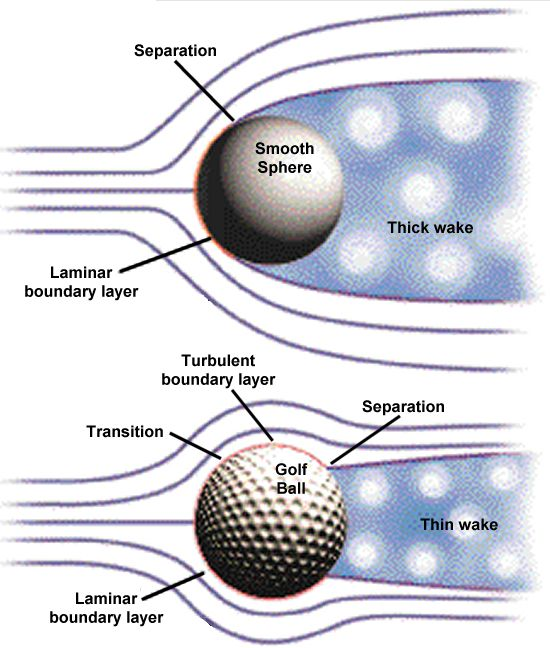
\includegraphics[scale = 0.2]{dimpled.jpg}
      \caption{Bola de golf vs bola suave.}
    \end{figure}
\end{frame}

%%%%%%%%%%%%%%%%%%%%%%%5
\begin{frame}{Dinámica traslacional}
\framesubtitle{Crisis de arrastre}
	\begin{figure}[H]
      \centering
      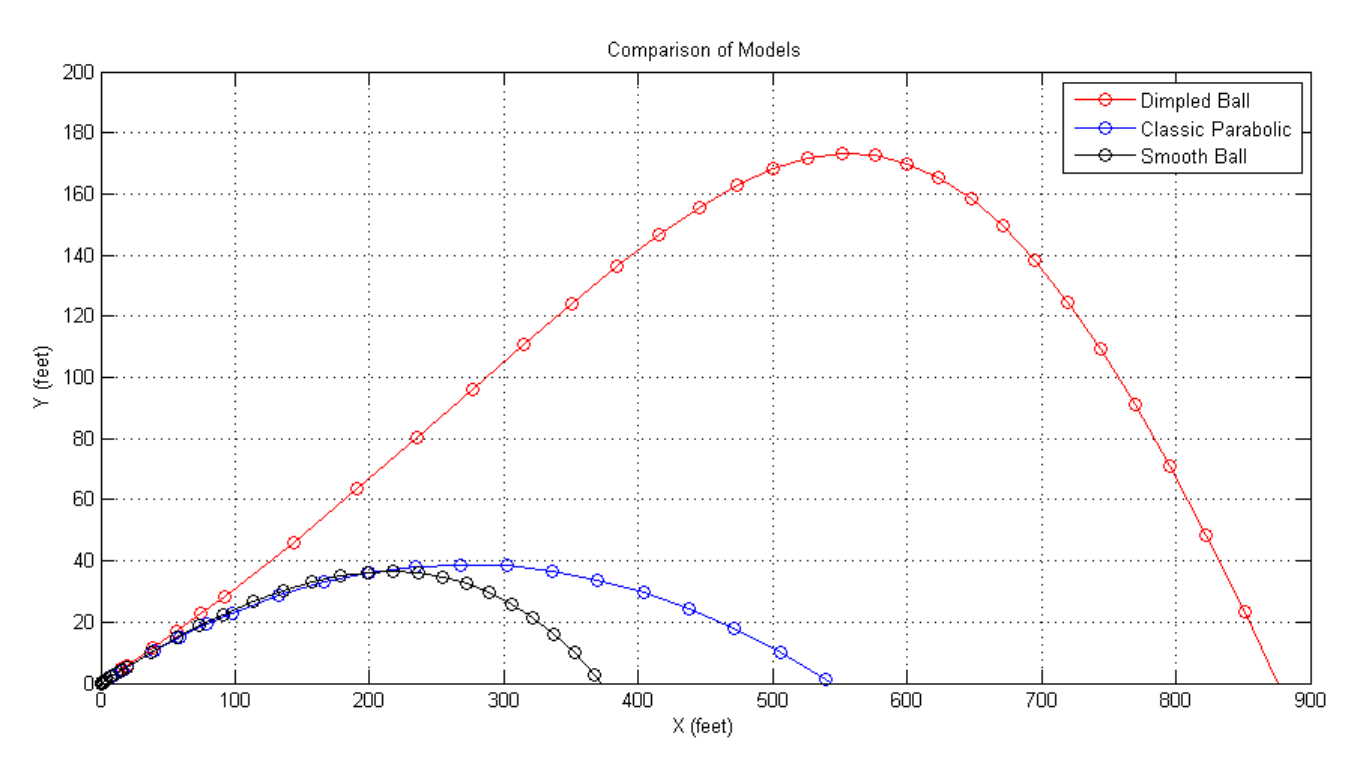
\includegraphics[scale = 0.2]{Comp.png}
      \caption{Bola de golf vs bola suave.}
    \end{figure}
\end{frame}
 %%%%%%%%%%%%%%%%%%%%%%%%%%%%%
 \subsection{Explicación de la crisis}
 \begin{frame}{DINÁMICA TRASLACIONAL}
 \framesubtitle{Explicación de la crisis}
 	\begin{itemize}
 	\item Turbulencia de la capa límite.
    \item Combinación de aire rápido y lento. 
    \item Separación de la capa límite.
    \item Reducción de la fuerza de arrastre
 	\end{itemize}
    \begin{figure}[H]
      \centering
      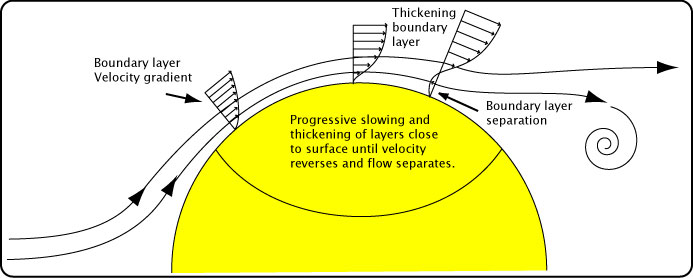
\includegraphics[scale = 0.3]{grad.jpg}
      \caption{Diagrama de cuerpo libre para una bola de golf\footnotemark{}.}
    \end{figure}
     \footnotetext{\bibentry{crisis}.}
 \end{frame}

%%%%%%%%%%%%%%%%%%%%%%%%%%%%%%%%%%%%%
 \subsection{Fuerzas ejercidas por el golfista}
 \begin{frame}{DINÁMICA TRASLACIONAL}
 \framesubtitle{Fuerzas ejercidas por el golfista}
 \textbf{- Reacción del piso:}
 	\begin{itemize}
 	\item $65\%$ del peso se encuentra sobre el pie trasero durante el backswing
    \item Transfieren rápidamente el peso de un pie a otro 
    \item El pico de mayor peso sobre el pie delantero se alcanza en la mitad del downswing
    \item Los jugadores con menos habilidades no transfieren tanto peso de un pie a otro y lo hacen de manera más lenta.
 	\end{itemize}
    \begin{figure}[H]
      \centering
      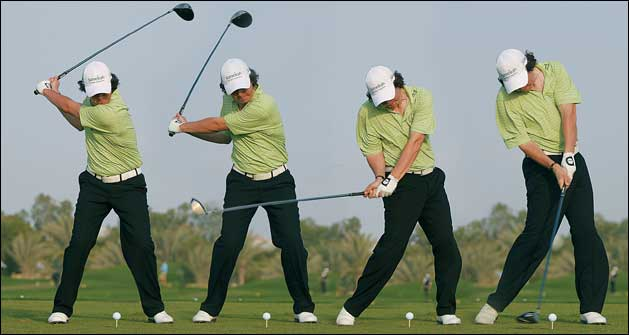
\includegraphics[scale = 0.25]{player.jpg}
      \caption{Jugador realizando un swing\footnotemark{}.}
     \end{figure}
     \vspace{-2cm}\footnotetext{\bibentry{player}.}
\end{frame}
%%%%%%%%%%%%%%%%%%%%%%%%%%%%%%%%%%%%%%
\begin{frame}{DINÁMICA TRASLACIONAL}
\framesubtitle{Fuerzas Musculares}
Los jugadores más avanzados utilizan los grades músculos de las piernas y las caderas para obtener más potencia, mientras que los que tienen menos habilidades requieren más fuerza en brazos y espalda.
\begin{figure}
  \centering
  \begin{subfigure}[H]{0.3\textwidth}
    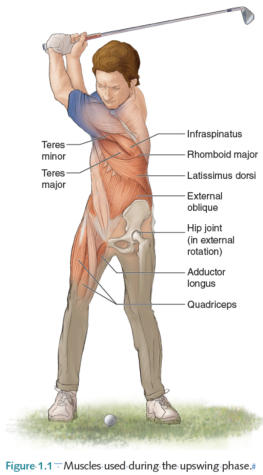
\includegraphics[scale = 0.25]{body1.jpg}
    \centering
    %\caption{Paisaje 1.}
  \end{subfigure}
  \hspace{-1cm} % Add desired spacing between images, e. g. ~, \quad, \qquad, \hfill etc (or a blank line to force the subfigure onto a new line)
  \begin{subfigure}[H]{0.3\textwidth}
    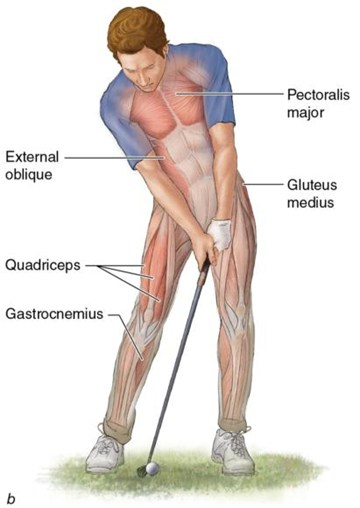
\includegraphics[scale = 0.25]{body2.jpg}
    \centering
    %\caption{}
  \end{subfigure} % a spacing can be put before caption
  \vspace{-2mm}
  \caption{Músculos utilizados durante un swing\footnotemark{}.}
\end{figure}
\footnotetext{\bibentry{body}}
\end{frame}



\section{CINEMÁTICA}
\subsection{Parabólico Tradicional}
\begin{frame}{CINEMÁTICA}
	\framesubtitle{Parabólico Tradicional}
	\begin{equation}
	x\left( t \right)=-v_{0}\cos \theta t+x_{0}
	\end{equation}
    \begin{equation}
    y(t)=-\frac { 1 }{ 2 } g{ t }^{ 2 }+{ v }_{ 0 }\sin { \theta t+{ y }_{ 0 } }
    \end{equation}
    \begin{equation}
    y\left( x \right)=y_{0}+x\tan \theta -\frac{g}{2v_{0}^{2}\cos ^{2}\theta }x^2
    \end{equation}
	\begin{figure}[H]
  		\centering
  		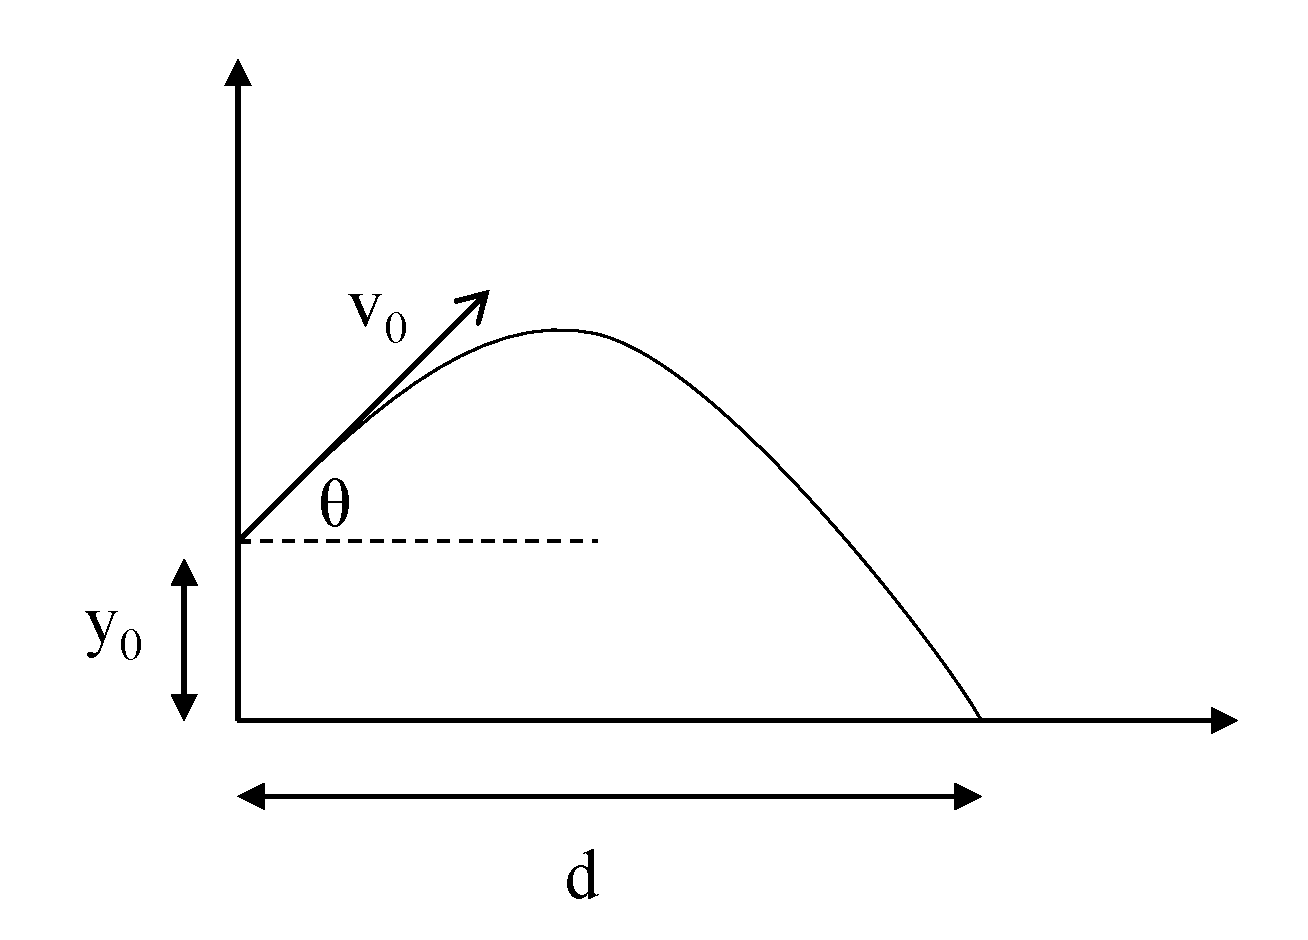
\includegraphics[scale = 0.2]{Motion.eps}
 		\caption{Movimiento parabólico.}
	\end{figure}
\end{frame}
%%%%%%%%%%%%%%%%%%%%%%%%%%
\subsection{Resistencia Simple al Aire}
\begin{frame}{CINEMÁTICA}
\framesubtitle{Resistencia Simple al Aire}
	\begin{equation}
    \begin{gathered}
	\Sigma F_y = -mg -kv_{y} = ma_y\\
    \Sigma F_x = -kv_{x} = ma_x
    \end{gathered}
	\end{equation}
	\begin{figure}[H]
  		\centering
  		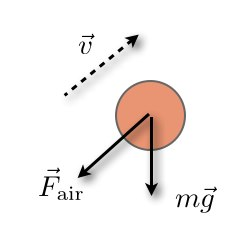
\includegraphics[scale = 0.4]{fbdBall.jpg}
 		\caption{Diagrama de cuerpo libre para una bola con resistencia simple al aire.}
	\end{figure}
\end{frame}
%%%%%%%%%%%%%%%%%%%%%%%%
\begin{frame}{CINEMÁTICA}
\framesubtitle{Resistencia Simple al Aire}
\begin{equation}
x\left( t \right)=x_{0}-\frac{v_{ox}m}{k}e^{-\frac{k}{m}t;}
\end{equation}
\begin{equation}
	y\left( t \right)=y_{0}-\frac{m}{k}\left[ gt+\left( v_{0y}+\frac{mg}{k} \right)e^{-\frac{k}{m}t} \right]
\end{equation}
\begin{equation}
	y\left( x \right)=\frac{m^{2}g}{k^{2}}\ln \left( -\frac{k}{mv_{0y}}x \right)+\left( 1+\frac{mg}{kv_{0x}} \right)
\end{equation}
	\begin{figure}[H]
  		\centering
  		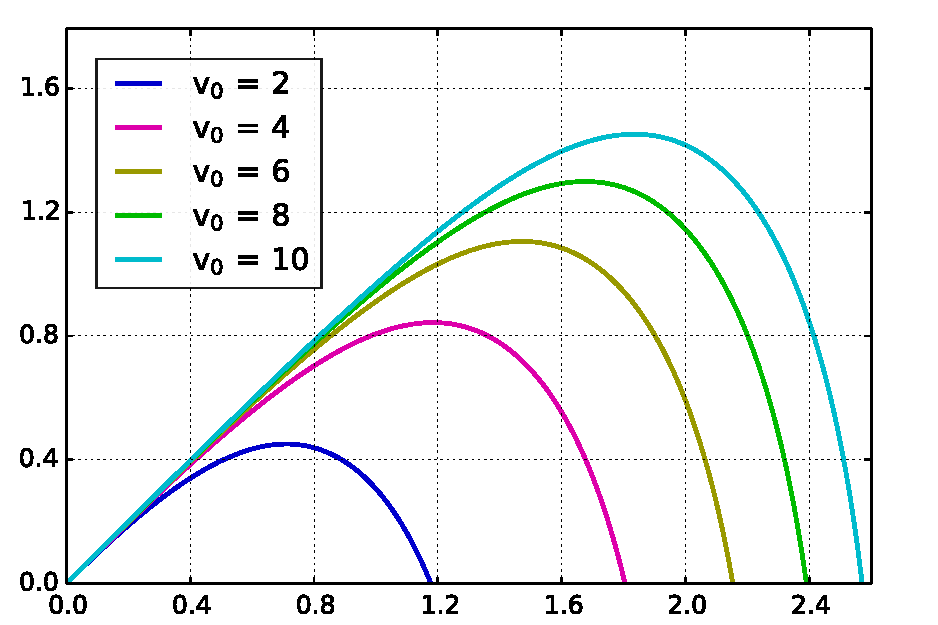
\includegraphics[scale = 0.3]{balistico.pdf}
 		\caption{Movimiento de un objeto con resistencia al aire para diferentes velocidades iniciales\footnotemark{}.}
	\end{figure}
    \vspace{-1cm}\footnotetext{\bibentry{airRes}}
    \footnotetext{Simulación: \url{https://www.geogebra.org/m/rYmNxYMY}}
\end{frame}

%%%%%%%%%%%%%%%%%%%%%%%%%%%%%%%%%%%%%%%%%%%%%%%%%
\subsection{Ecuación de Navier-Stokes}
\begin{frame}{CINEMÁTICA}
\framesubtitle{Ecuación de Navier-Stokes}
\url{https://www.youtube.com/watch?v=azyN4CXCiEE}
\begin{equation}
\rho \left( \frac{\partial u}{\partial t}+u\cdot\nabla\; u \right)=-\nabla\; p+\nabla\cdot\left( \mu \left( \nabla\; u\; +\; \left( \nabla\; u \right)^{T} \right)-\frac{2}{3}\mu \left( \nabla\cdot\; u \right)I \right)+\rho g+F
\end{equation}
	\begin{figure}[H]
  		\centering
  		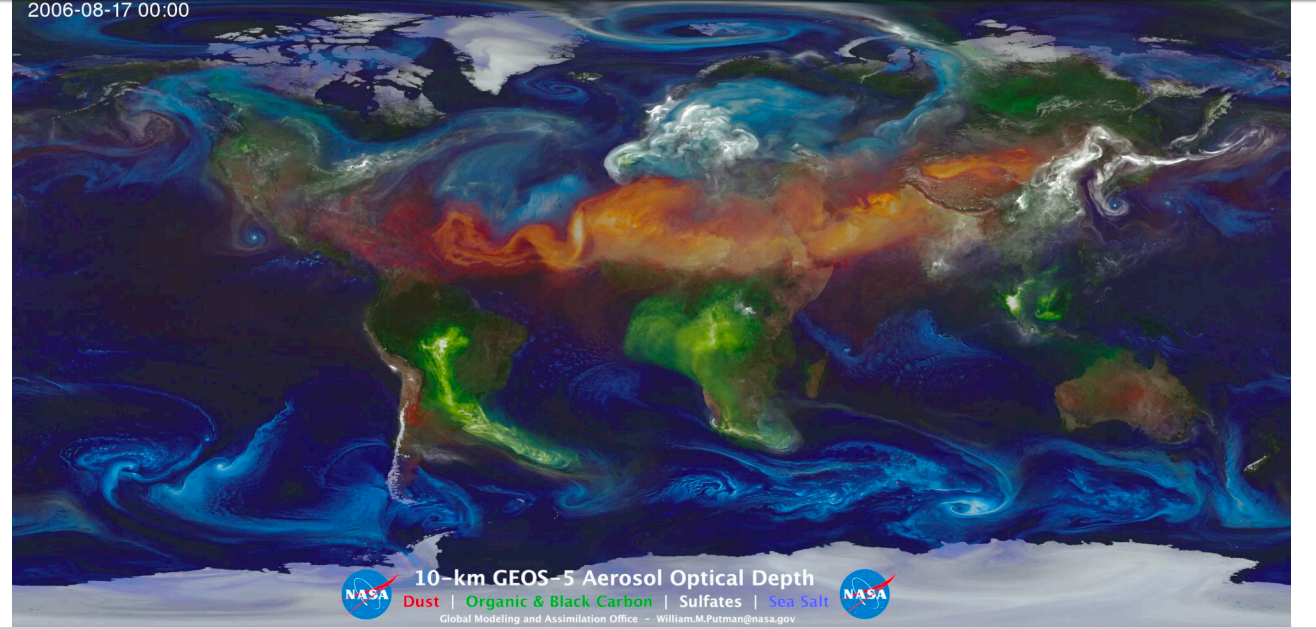
\includegraphics[scale = 0.2]{Navier.png}
 		\caption{Dinámica de fluidos.}
	\end{figure}
\end{frame}

\section{DINÁMICA ROTACIONAL}
\subsection{Análisis de Torque}
\begin{frame}{DINÁMICA ROTACIONAL}
\framesubtitle{Análisis de Torque}
	En el golf podemos evidenciar rotación en cuatro partes:
    \begin{itemize}
    \item Rotación bola de golf.
    \item Rotación palo y brazos.
    \item Rotación de las caderas.
    \item Rotación de las piernas.
    \end{itemize}

	\begin{figure}[H]
      \centering
      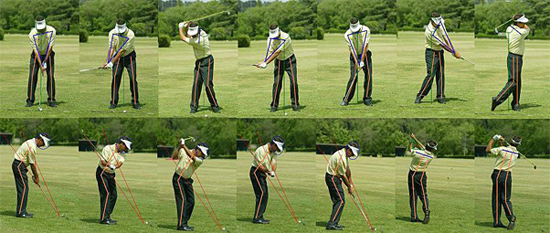
\includegraphics[scale = 0.375]{Swing.jpg}
      \caption{Movimiento durante un swing\footnotemark{}.}
    \end{figure}
     \vspace{-2cm}\footnotetext{\bibentry{swing1}.}
\end{frame}

%%%%%%%%%%%%%%%%%%%%%%%%%%%%
\subsection{Torque palo de golf}
\begin{frame}{DINÁMICA ROTACIONAL}
\framesubtitle{Torque palo de golf}
Para analizar dicho torque, hay que tener en cuenta:\begin{itemize}
\item Eje de rotación
\item El sistema
\end{itemize}
\begin{figure}[H]
      \centering
      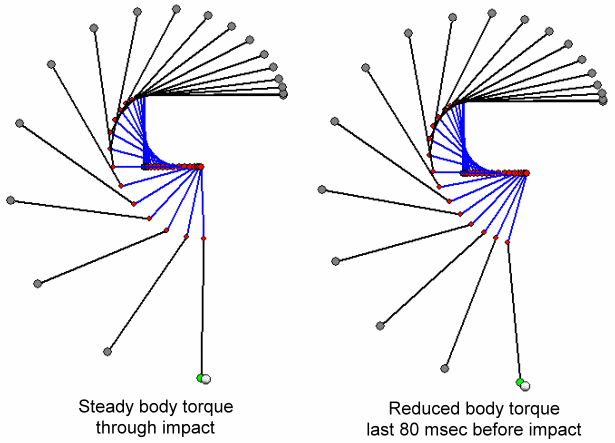
\includegraphics[scale = 0.275]{Movement_body.jpg}
      \caption{Sistema rotacional para el torque.}
\end{figure}
\end{frame}

%%%%%%%%%%%%%%%%%%%%%%%%%%%%%
\begin{frame}{DINÁMICA ROTACIONAL}
\framesubtitle{Torque palo de golf}
Con todo lo dicho, podriámos considerar el sistema como un péndulo doble.
\begin{figure}[H]
      \centering
      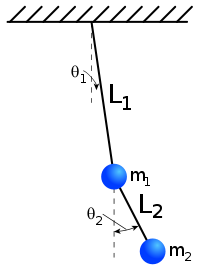
\includegraphics[scale = 0.3]{Double_Pendulum.png}
      \caption{Sistema de péndulo doble.}
\end{figure}
\begin{equation}
\alpha =\frac { 2\sin { ({ \theta  }_{ 1 }-\theta )\left( { { c }_{ 1 } }{ \omega  }_{ 1 }^{ 2 }+c_{ 2 }\cos { { \theta  }_{ 1 } } +{ c }_{ 3 }{ \omega  }^{ 2 }\cos { \left( { { \theta  }_{ 1 }-\theta  } \right)  }  \right)  }  }{ { c }_{ 4 }-{ c }_{ 5 }\cos { (2\left( { \theta  }_{ 1 }-\theta  \right) ) }  } 
\end{equation}
\end{frame}
%%%%%%%%%%%%%%%%%%%%%%%%%%%%%%%%%%%%%%%%%%%%%%%%%
\subsection{Efecto Magnus}
\begin{frame}{DINÁMICA ROTACIONAL}
\framesubtitle{Efecto Magnus}
\url{https://www.youtube.com/watch?v=2OSrvzNW9FE}\quad(0:00 - 1:24).
\begin{figure}[H]
      \centering
      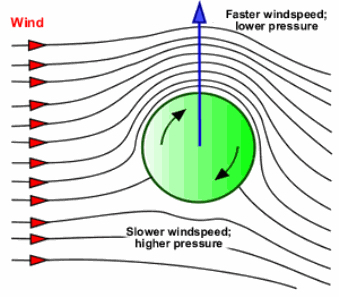
\includegraphics[scale = 0.3]{Magnus.jpg}
      \caption{Efecto magnus en un cuerpo esférico.}
\end{figure}
\begin{equation}
\frac { 1 }{ 2 } \rho { v }^{ 2 }+\rho gh+P=Cte
\end{equation}
\end{frame}
%%%%%%%%%%%%%%%%%%%%%%%%%%%%%%%%%%%%%%%%%%%%%%
\begin{frame}{DINÁMICA ROTACIONAL}
\framesubtitle{Efecto Magnus}
Para una esfera, la fuerza que hace este efecto sería apróximadamente:
\begin{equation}
\vec { F } \approx \left( { \pi  }^{ 2 }{ r }^{ 3 }\rho  \right) \vec { \omega  } \times \vec { v } 
\end{equation}
\begin{figure}[H]
      \centering
      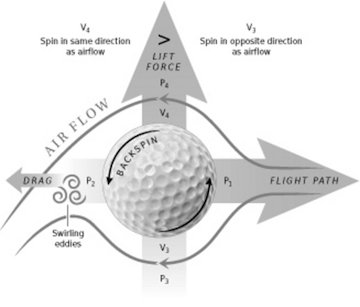
\includegraphics[scale = 0.385]{Golf_Magnus.jpg}
      \caption{Efecto magnus en un cuerpo esférico.}
\end{figure}
\end{frame}
%%%%%%%%%%%%%%%%%%%%%%%%%%%%%%%%%%%%%%%%%%%%%
\subsection{Torque bola de golf}
\begin{frame}{DINÁMICA ROTACIONAL}
\framesubtitle{Torque bola de golf}
Hay tres tipos de rotaciones con efectos positivos y una con efectos negativos.
\begin{itemize}
	\item Hook
	\item Slice
	\item Backspin
	\item \textbf{Overspin}
\end{itemize}
\end{frame}
\section{ACCESORIOS Y CARACTERÍSTICAS}
\subsection{Palos de golf}
\begin{frame}{ACCESORIOS Y CARACTERÍSTCAS}
\framesubtitle{Palos de golf: maderas}
	Son los palos con los que se puede golpear más fuertemente y lograr mayor distancia.
	\begin{figure}[H]
      \centering
      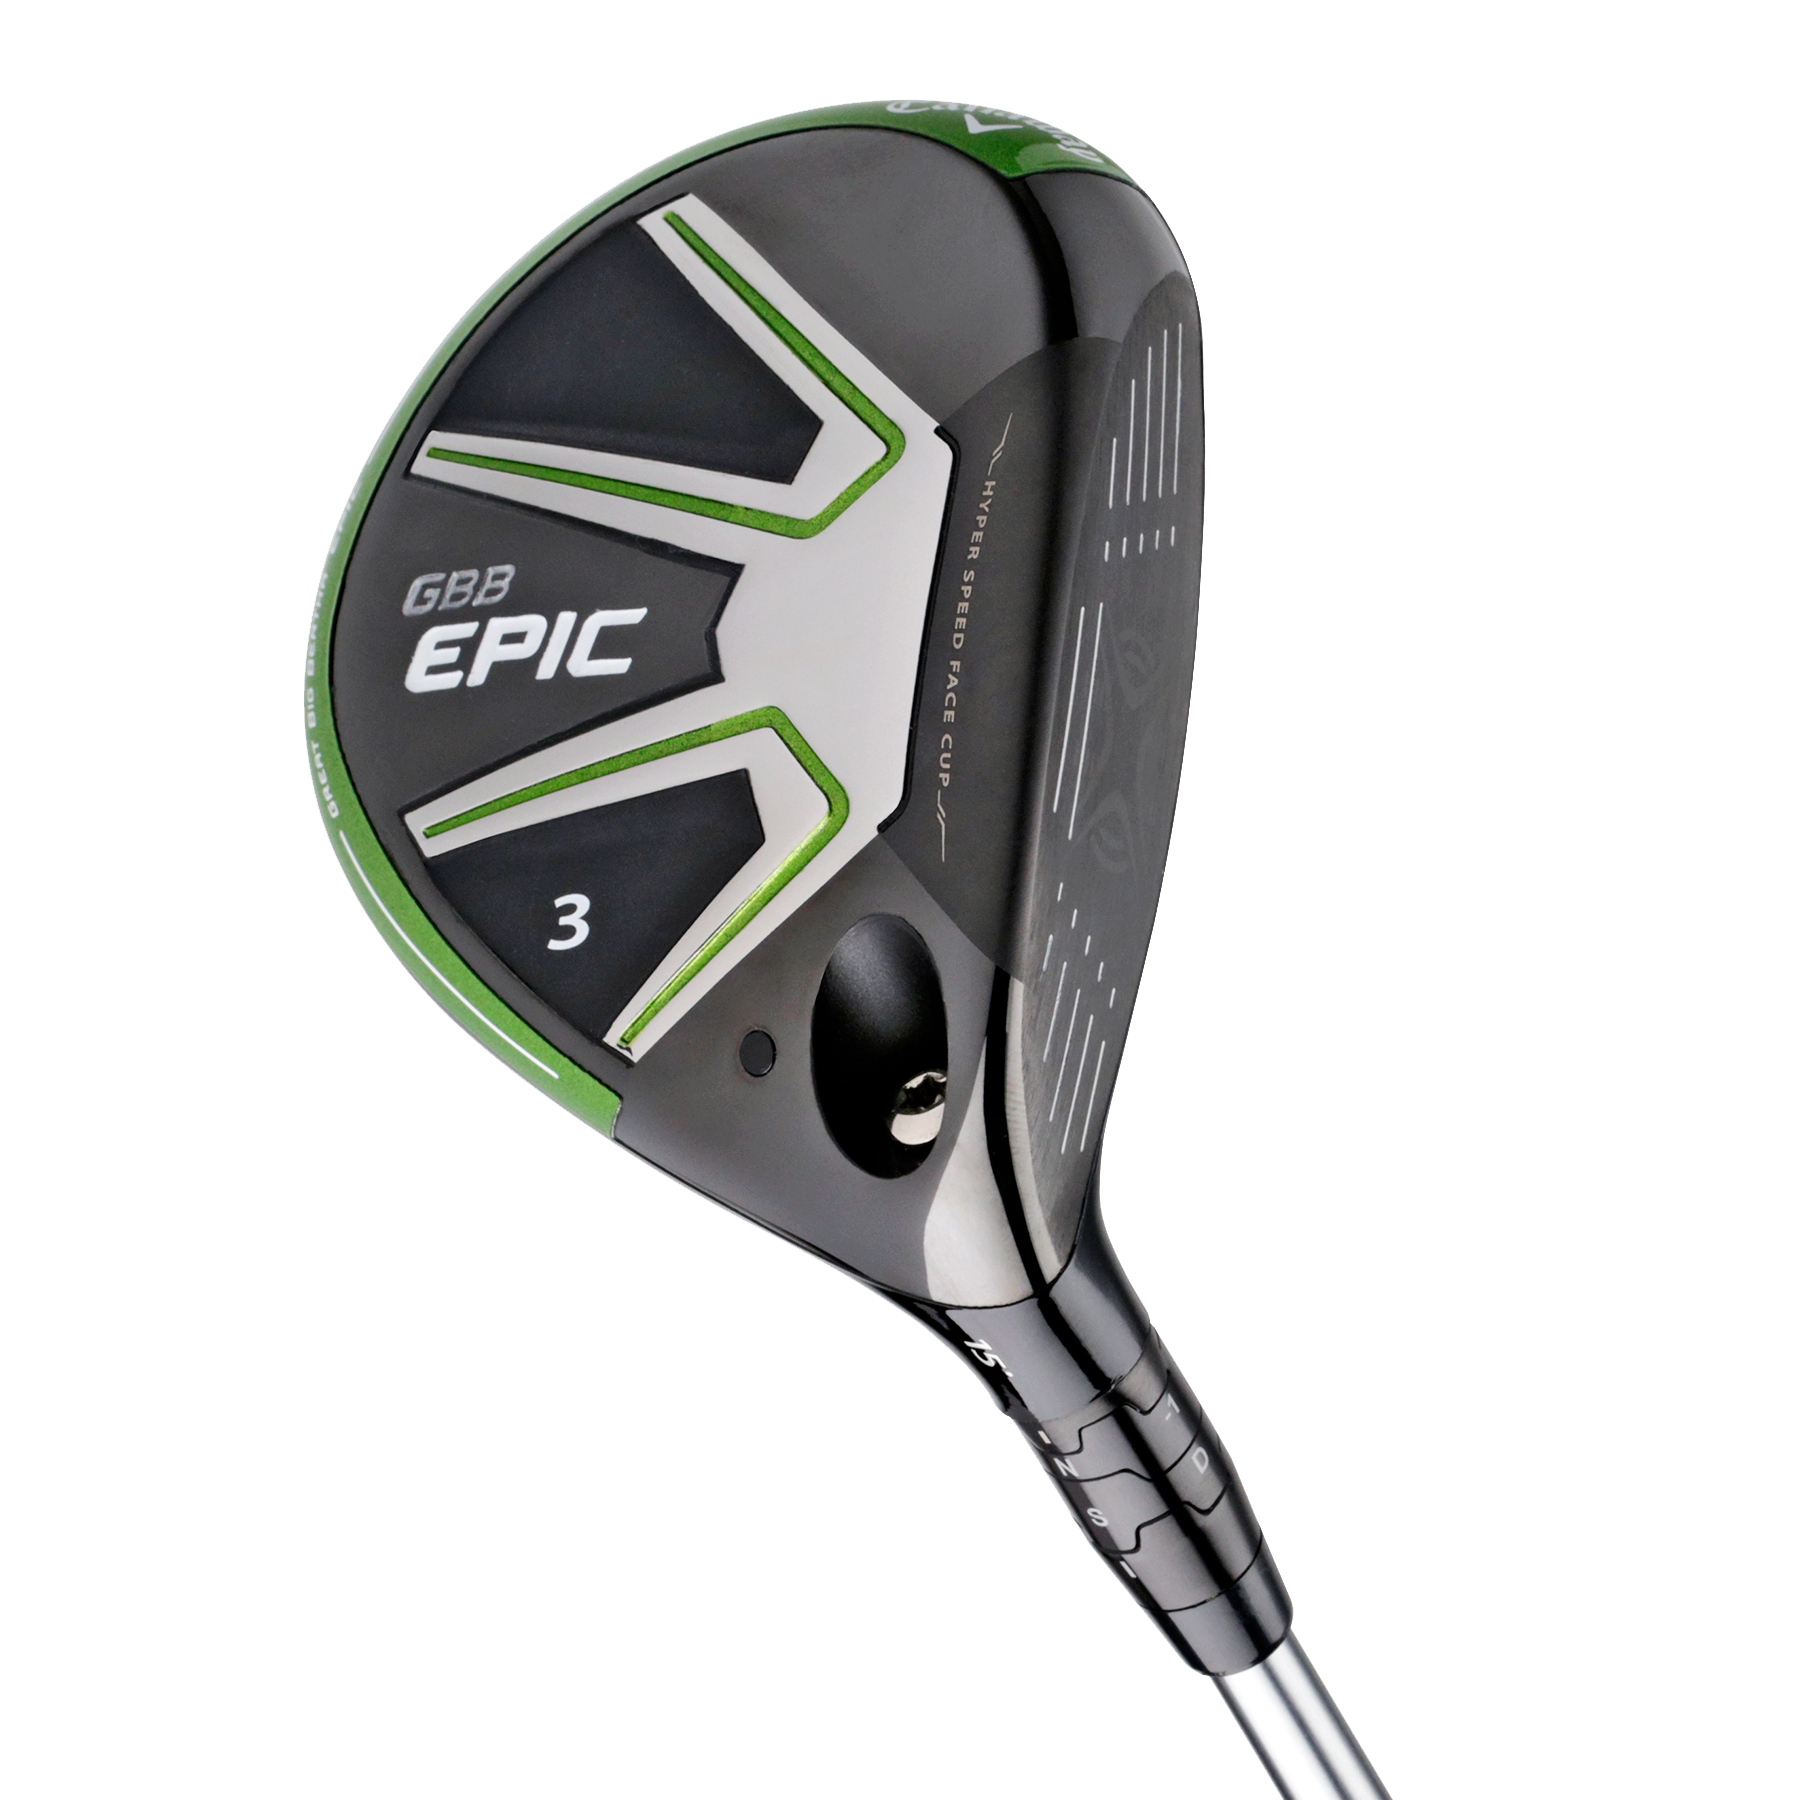
\includegraphics[scale = 0.075]{woods.png}
      \caption{Palo madera\footnotemark{}.}
	\end{figure}
    \footnotetext{\bibentry{woods}}
\end{frame}
%%%%%%%%%%%%%%%%%%%%%%
\begin{frame}{ACCESORIOS Y CARACTERÍSTICAS}
\framesubtitle{Palos de golf: wedge}
En éstos se consigue un mejor control de la bola, usualmente útil para situaciones difíciles.
	\begin{figure}[H]
      \centering
      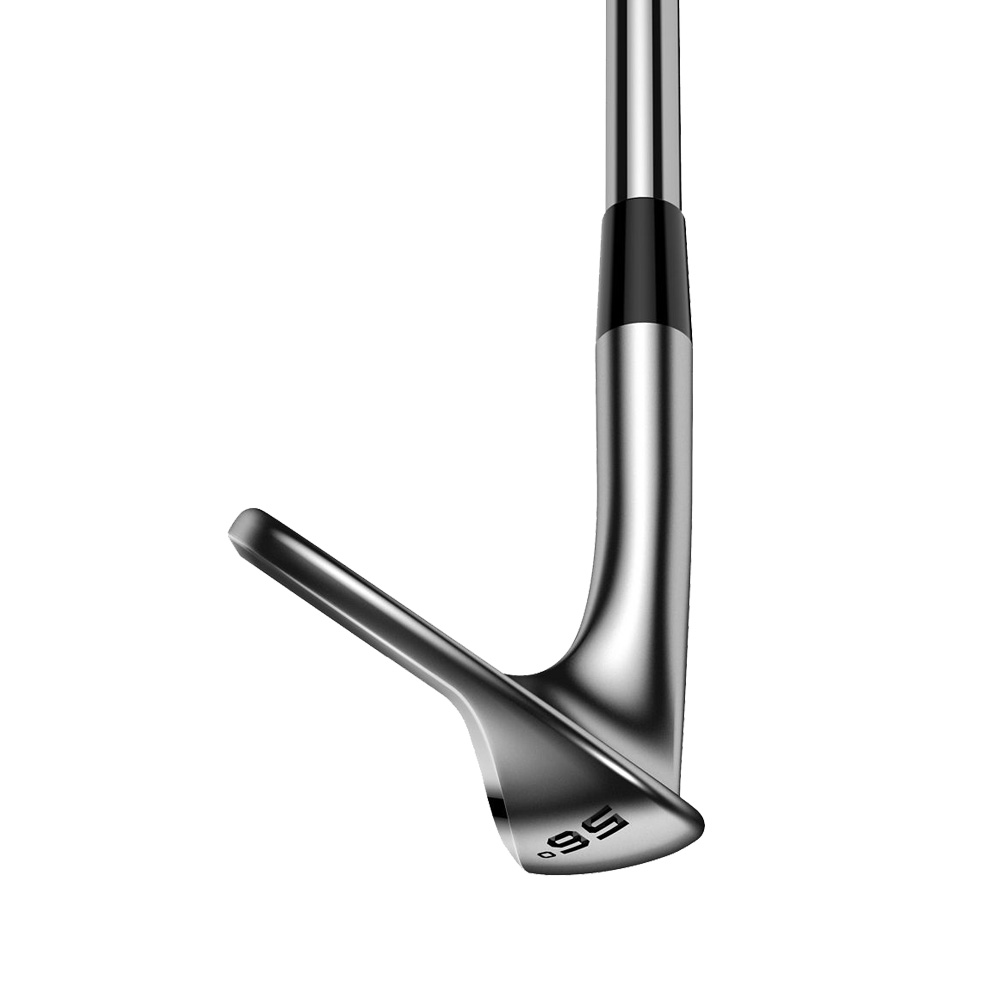
\includegraphics[scale = 0.125]{wedge.jpg}
      \caption{Palo wedge/iron\footnotemark{}.}
	\end{figure}
\vspace{-2cm}\footnotetext{\bibentry{wedge}}
\end{frame}

%%%%%%%%%%%%%%%%%%%%%%%
\begin{frame}{ACCESORIOS Y CARACTERÍSTICAS}
\framesubtitle{Palos de golf: putter}
Finalmente se utiliza un palo denominado putter para empujar la bola mediante un golpe (putt) hacia el hoyo en el green.
	\begin{figure}[H]
      \centering
      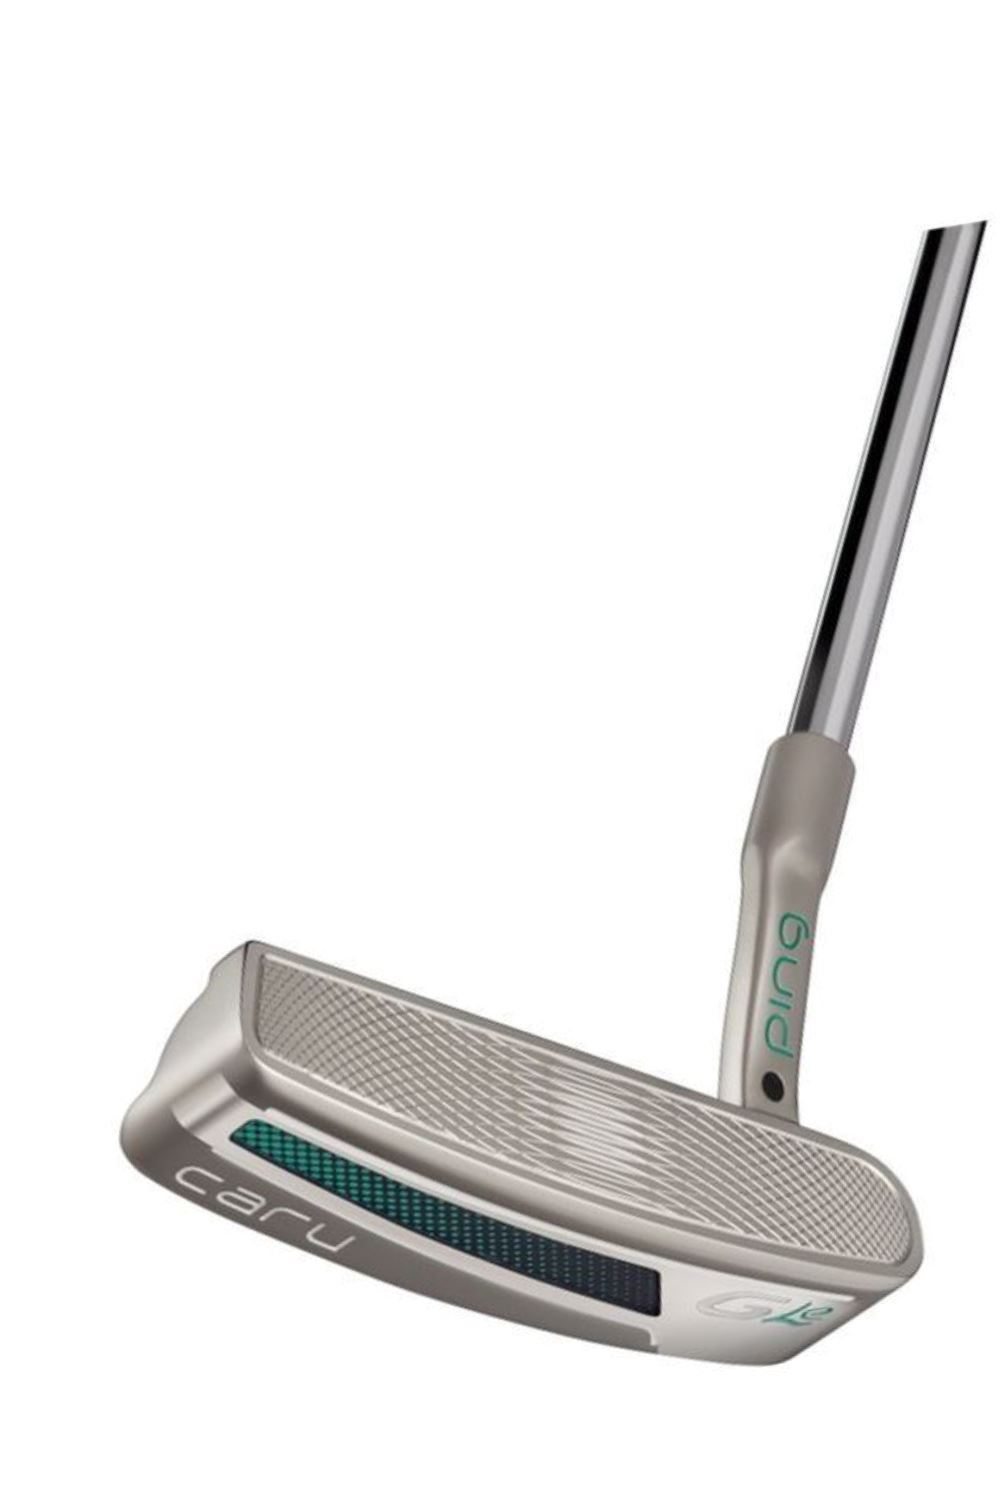
\includegraphics[scale = 0.125]{putter.jpeg}
      \caption{Palo putter\footnotemark{}.}
	\end{figure}
	\vspace{-1cm}\footnotetext{\bibentry{putter}}
\end{frame}

\section{CONCLUSIONES}
\begin{frame}{CONCLUSIONES}
\begin{itemize}
\item Se logró describir (más que analizar) la cinemática, dinámica traslacional y rotacional en el golf desde diferentes perspectivas físicas (por ejemplo, para la cinemática se describieron tres modelos de movimiento de la bola); aunque no se lograron explicar a fondo algunos de los fenómenos aquí descritos, creemos que se logró una exposición con un enfoque más motivador e informativo.
\end{itemize}
\end{frame}
\nonumb % Not numbered titles
%\addcontentsline{toc}{section}{\small\protect\numberline{}{REFERENCIAS BIBLIOGRÁFICAS}} % Separated from other contents, for small number of contents
\addcontentsline{toc}{section}{\small REFERENCES} % Closer from other contents, for large number of contents
\nocite{*} % All citations showed (take care with fraud!)
%%%%%%%%%%%%%%%%%%%%%%%%%%%%%%%%%%%%%%%%%%%%%%%%%%%%%%%%%%%%%%%%%%%%%%%%%%%%
\section*{REFERENCES}
\begin{frame}[allowframebreaks]{REFERENCES} %  and put before {REFEREN...}
\begingroup % Group for changing the color
\renewcommand{\color}[1]{} % Allows to have black bibs and white footnote bibs
\small{\bibliographystyle{IEEEtran}} % Size of text; acm or gatech-thesis or ieeetr or ieeetran or icontec or iso690
\bibliography{ref}
\endgroup % Group for changing the color
% pdflatex -> bibtex -> pdflatex -> pdflatex
\end{frame}
%%%%%%%%%%%%%%%%%%%%%%%%%%%%%%%%%%%%%%%%%%%%%%%%%%%%%%%%%%%%%%%%%%%%%%%%%%%%
% Thank-slide
\begin{frame}[plain,noframenumbering] % No frame number
	\begin{beamercolorbox}[ht=\paperheight,wd=\paperwidth, center]{Portada}
		\begin{center}\Huge\textbf{Thank you}\end{center} % Or Thanks; leave the next space mandatorily
		
		\vspace{0.44\paperheight}
    \end{beamercolorbox}
\end{frame}
%%%%%%%%%%%%%%%%%%%%%%%%%%%%%%%%%%%%%%%%%%%%%%%%%%%%%%%%%%%%%%%%%%%%%%%%%%%%


\end{document}
